\documentclass[table,dvipsnames]{beamer}
\mode<presentation>{
	\usetheme{Madrid}
	\setbeamercolor{title}{fg=Black,bg=Blue!15}
	\setbeamercolor{frametitle}{fg=Black,bg=Blue!15}
	\setbeamercolor{block title}{fg=Black,bg=Blue!15}
	\setbeamercolor{block}{fg=Black,bg=Blue!10}
}

\usepackage{graphicx}
\usepackage{booktabs}
\usepackage{xcolor}
\usepackage{multirow}
\usepackage{minted}
\usepackage[
type={CC},
modifier={by-sa},
version={4.0},
]{doclicense}

\definecolor{LightGray}{gray}{0.9}

\title[Rangkuman Kegiatan]{Rangkuman Diskusi Usulan Pengujian Prototype ke PT. Global Quality Indonesia}
\author{}
\institute[VibrasticLab : \ccbysa]{
	Achmadi ST MT\\
	\medskip
	\textit{}
}
\date{}

\begin{document}

	\begin{frame}
		\titlepage
	\end{frame}

	\begin{frame}
		\frametitle{Pihak Yang Terlibat}

		\begin{exampleblock}{Perwakilan Tim Audiometri}
			Mas Achmadi, ST MT selaku prototype engineer dari Tim Audiometri
		\end{exampleblock}

		\begin{exampleblock}{Perwakilan PT Global Quality Indonesia}
			Bapak Eliyana Firmansyah, ST MT selaku Contact Person dari PT Global Quality Indonesia
		\end{exampleblock}

		\begin{exampleblock}{Tentang PT Global Quality Indonesia}
			PT. GLOBAL QUALITY INDONESIA is a limited partnership which its main businesses include provision of Calibration, Material Testing, Training, Quality Management Consultant and Maintenance services.
		\end{exampleblock}

		\begin{exampleblock}{Website PT Global Quality Indonesia}
			\url{https://www.globalquality.co.id/}
		\end{exampleblock}
	\end{frame}

	\begin{frame}
		\frametitle{Pertemuan Pertama}

		\begin{exampleblock}{Uraian Ringkas}
			Pertemuan offline pertama telah dilaksanakan di kantor PT Global Quality Indonesia yang beralamat KOPO MAS REGENSI BLOK N - No. 7 C Bandung-Indonesia,
			dengan menunjukkan prototype produk yang akan dilakukan pengujian.
		\end{exampleblock}

		\begin{exampleblock}{Dokumentasi}
			\begin{center}
				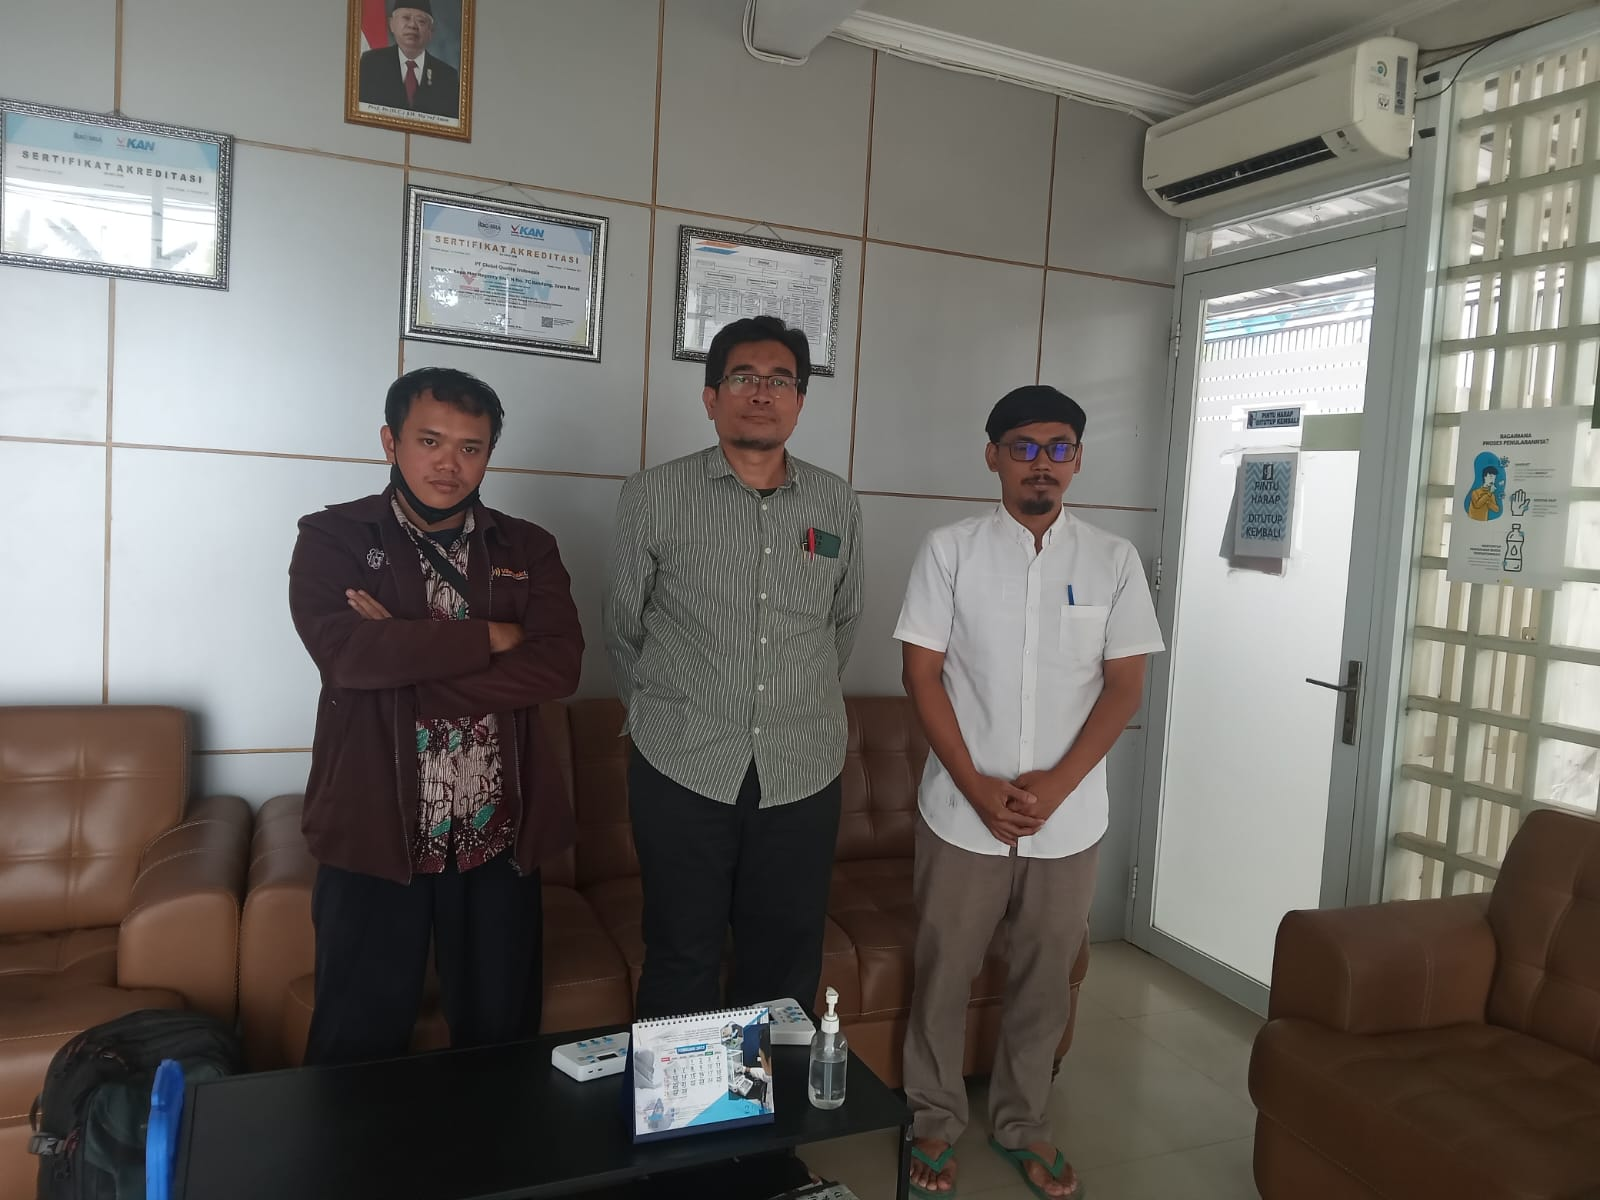
\includegraphics[width=150pt]{images/doc0}
			\end{center}
		\end{exampleblock}
	\end{frame}

\end{document}